This section provides the reader with an overview of the RV8 robot work cell. The primary operational aspects of the product, from the perspective of end users, maintainers and administrators, are defined here. The key features and functions found in the work cell, as well as critical user interactions are described in detail below.

\subsection{Features \& Functions}
The RV8 work cell will specialize in palletizing and depalletizing boxes. It will perform these operations through the use of a hydraulic gripper, vision sensors, and QR code scanners. The vertical robot initially has 6 axis, with a linear rail acting as the 7th axis. The robot will stack boxes on pallets, sorting the boxes through the use of scanner data. While performing the operation, several safety features will be implemented, such as emergency stops, industrial light towers, and presence detection within the work cell. The integrated components of the work cell are the programmable logic controller (PLC), host PC, and a CR800 handheld controller.

\subsection{External Inputs \& Outputs}
\begin{table}[H]
\resizebox{\textwidth}{!}{
\begin{tabular}{|l|l|l|l|}
\hline
 \textbf{Name} & \textbf{Description} & \textbf{Use}\\ \hline
 QR Code Scanner  & Application input & Scans the presence of boxes \\ \hline
 Presence Detection & System input & Detects motion within the work cell  \\ \hline
 Emergency Stops & User input & Stops the operation of the robot arm \\ \hline
 Industrial Light Tower  & System output & Indicates the state of the work cell  \\ \hline
 Raspberry Pi & I/O Logic & Handles the data from the QR code reader\\ \hline
\end{tabular}}
\caption{Overview of external inputs and outputs}
\end{table}

\subsection{Product Interfaces}
Specify what all operational (visible) interfaces look like to your end-user, administrator, maintainer, etc. Show sample/mocked-up screen shots, graphics of buttons, panels, etc. Refer to the critical external inputs and outputs described in the paragraph above.

\begin{figure}[h!]
	\centering
   	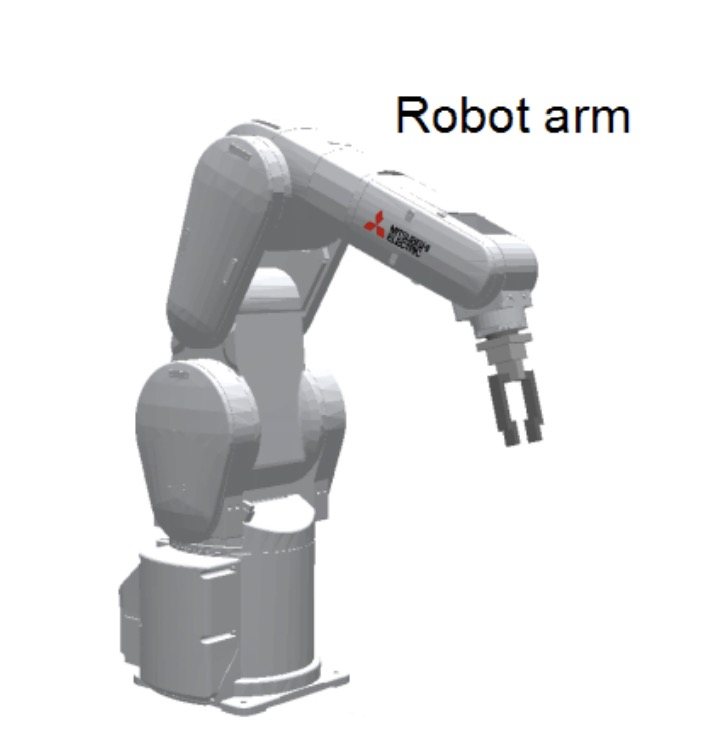
\includegraphics[width=0.30\textwidth]{images/RobotArm.jpg}
    \caption{Robot arm of RV8-CRL
    }
\end{figure}
\begin{figure}[h!]
	\centering
   	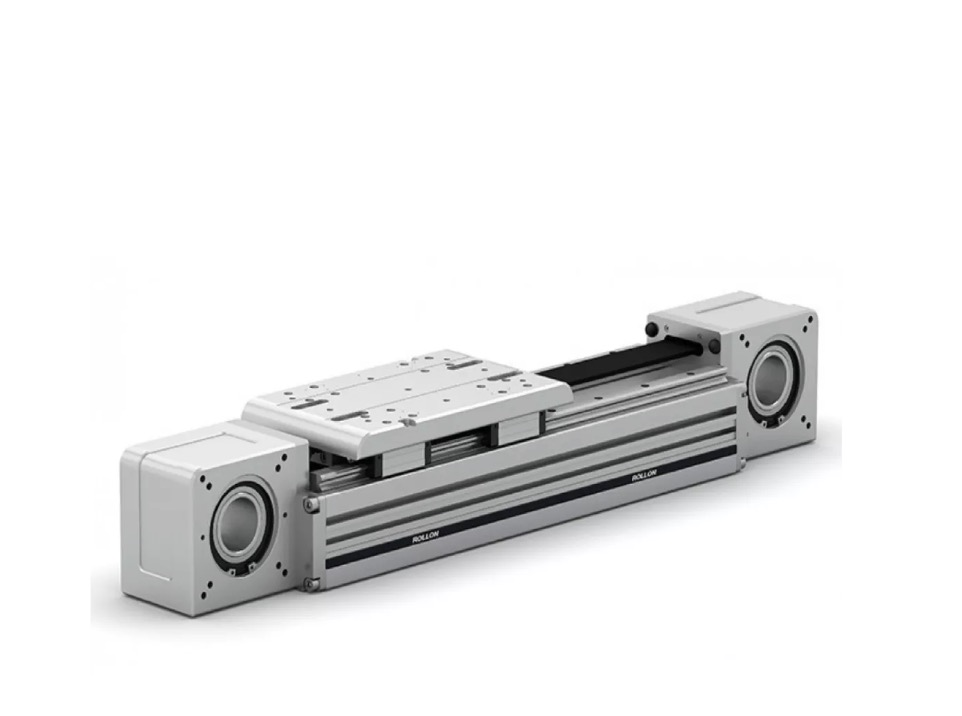
\includegraphics[width=0.40\textwidth]{images/LinearRail.jpg}
    \caption{Linear rail}
\end{figure}

\begin{figure}[h!]
	\centering
   	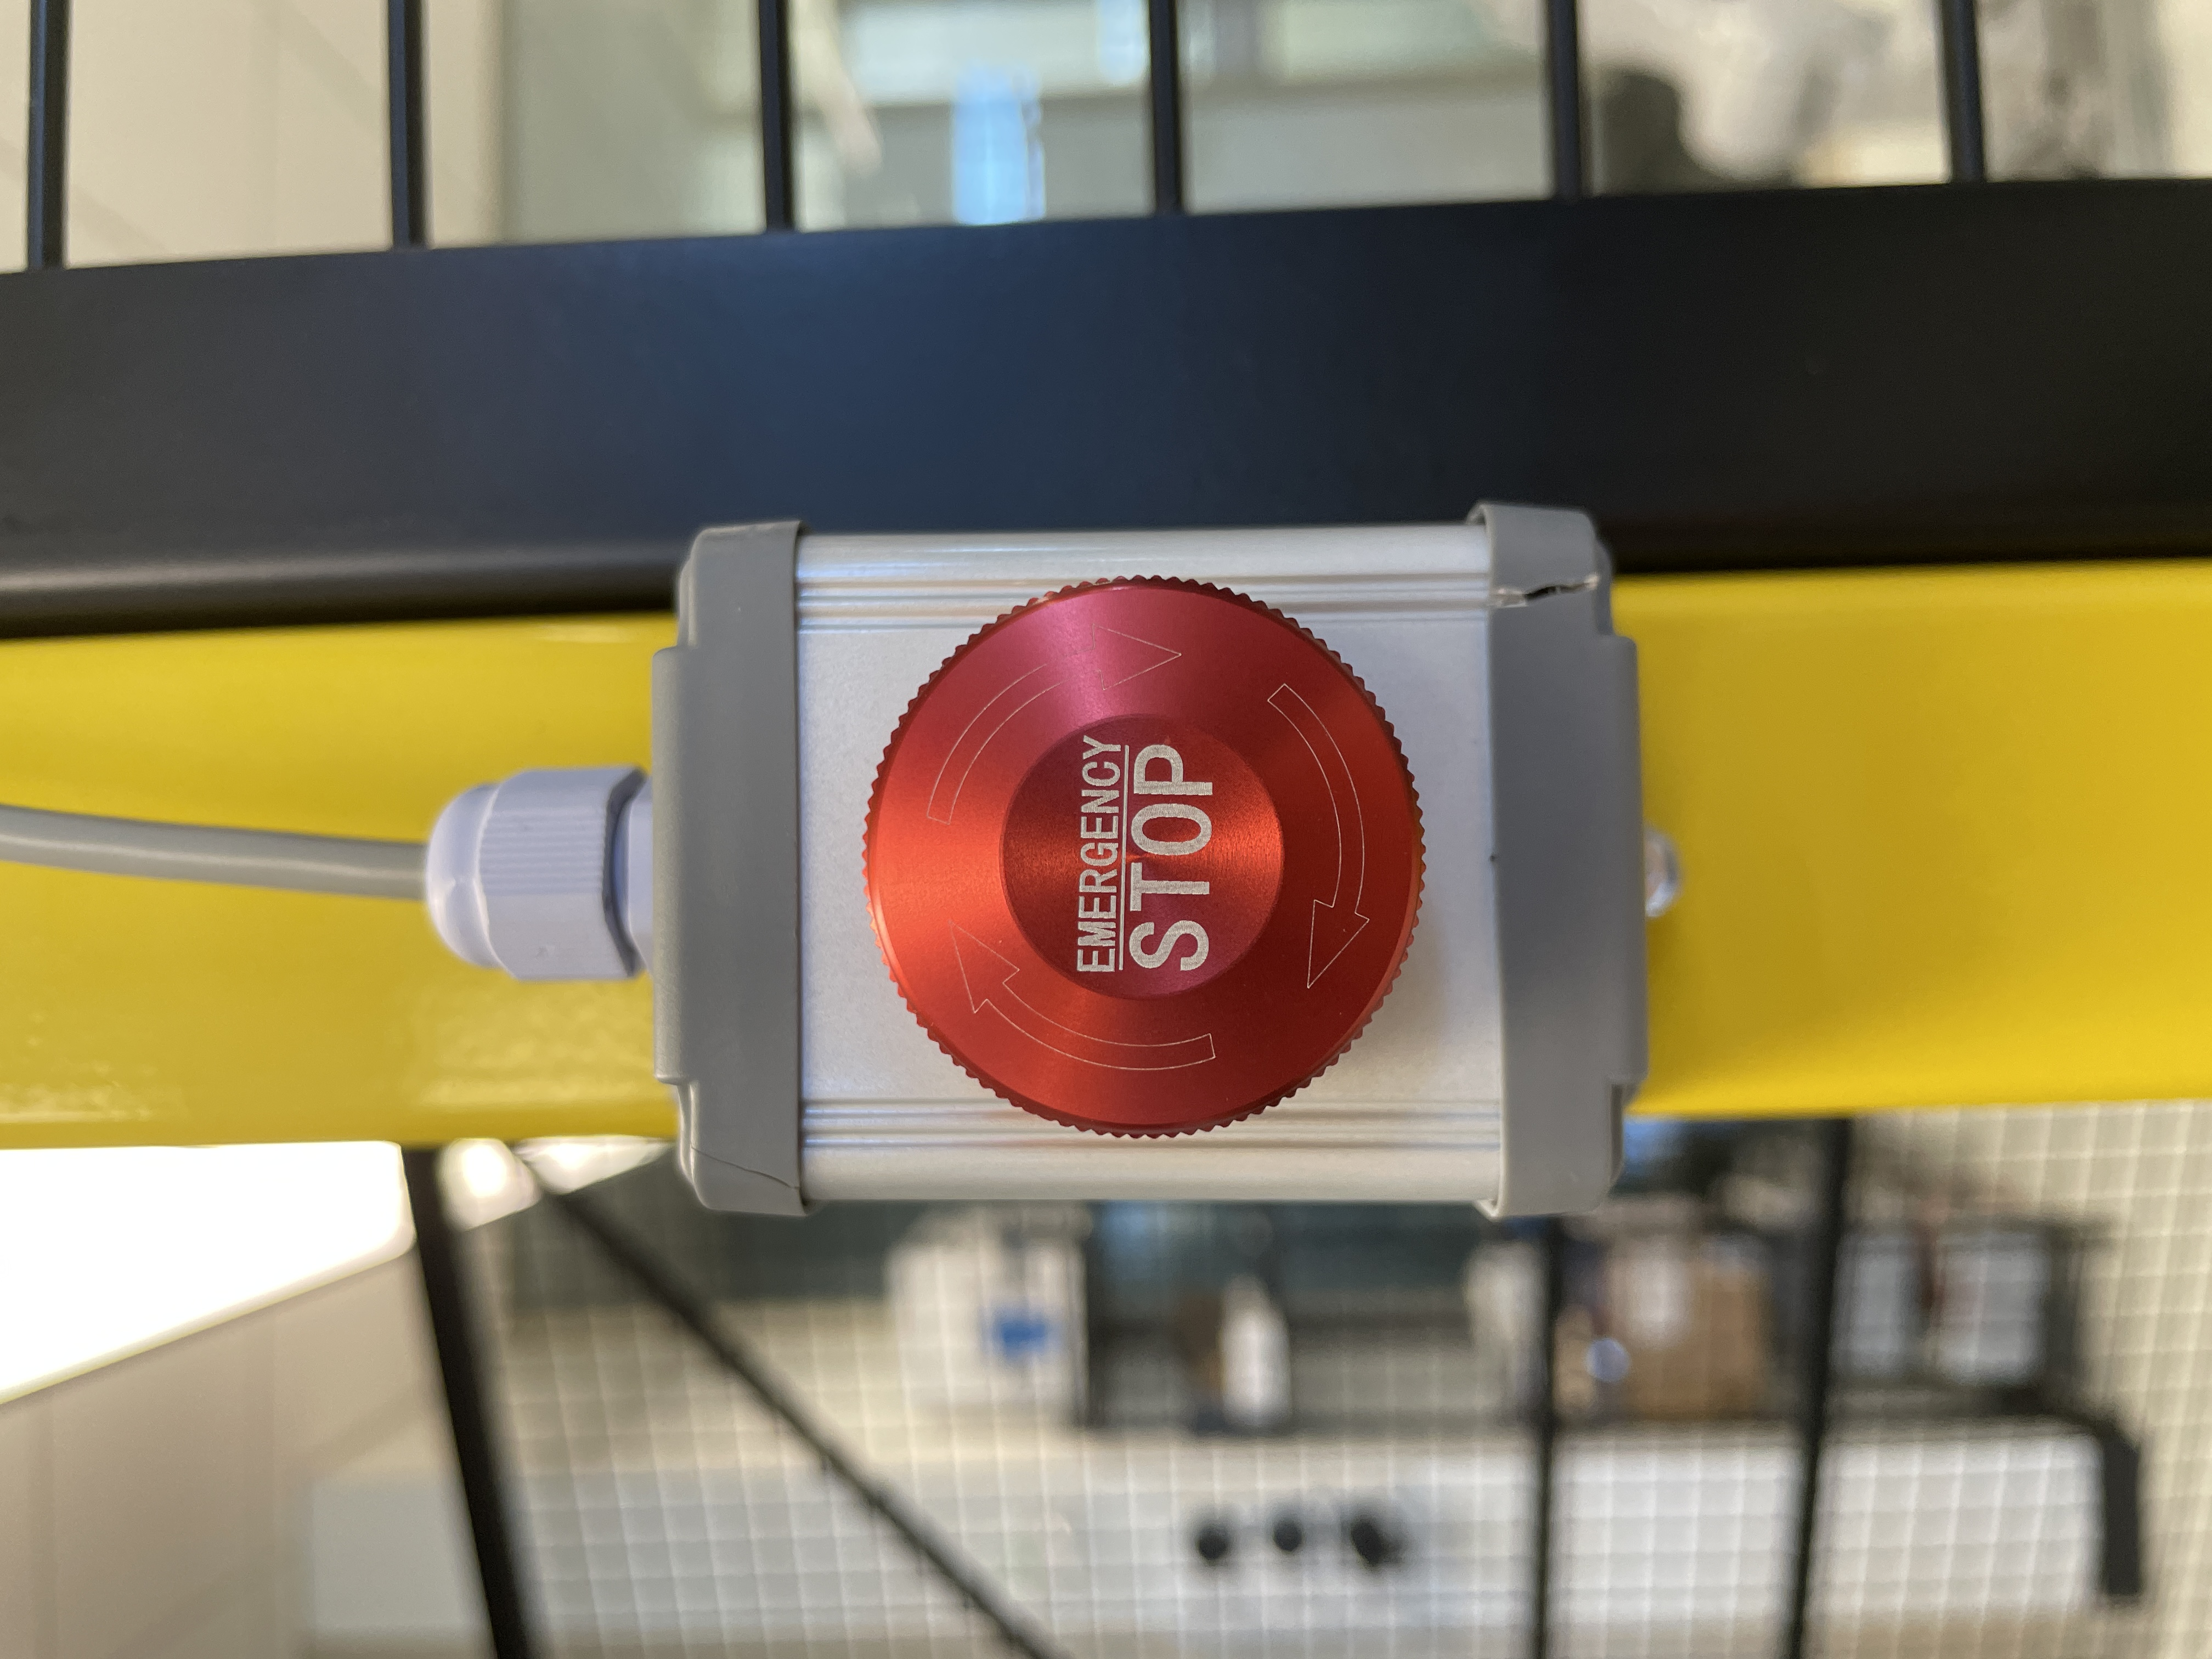
\includegraphics[width=0.40\textwidth, angle = -90]{images/EStop.JPG}
    \caption{Emergency stop}
\end{figure}

\begin{figure}[h!]
	\centering
   	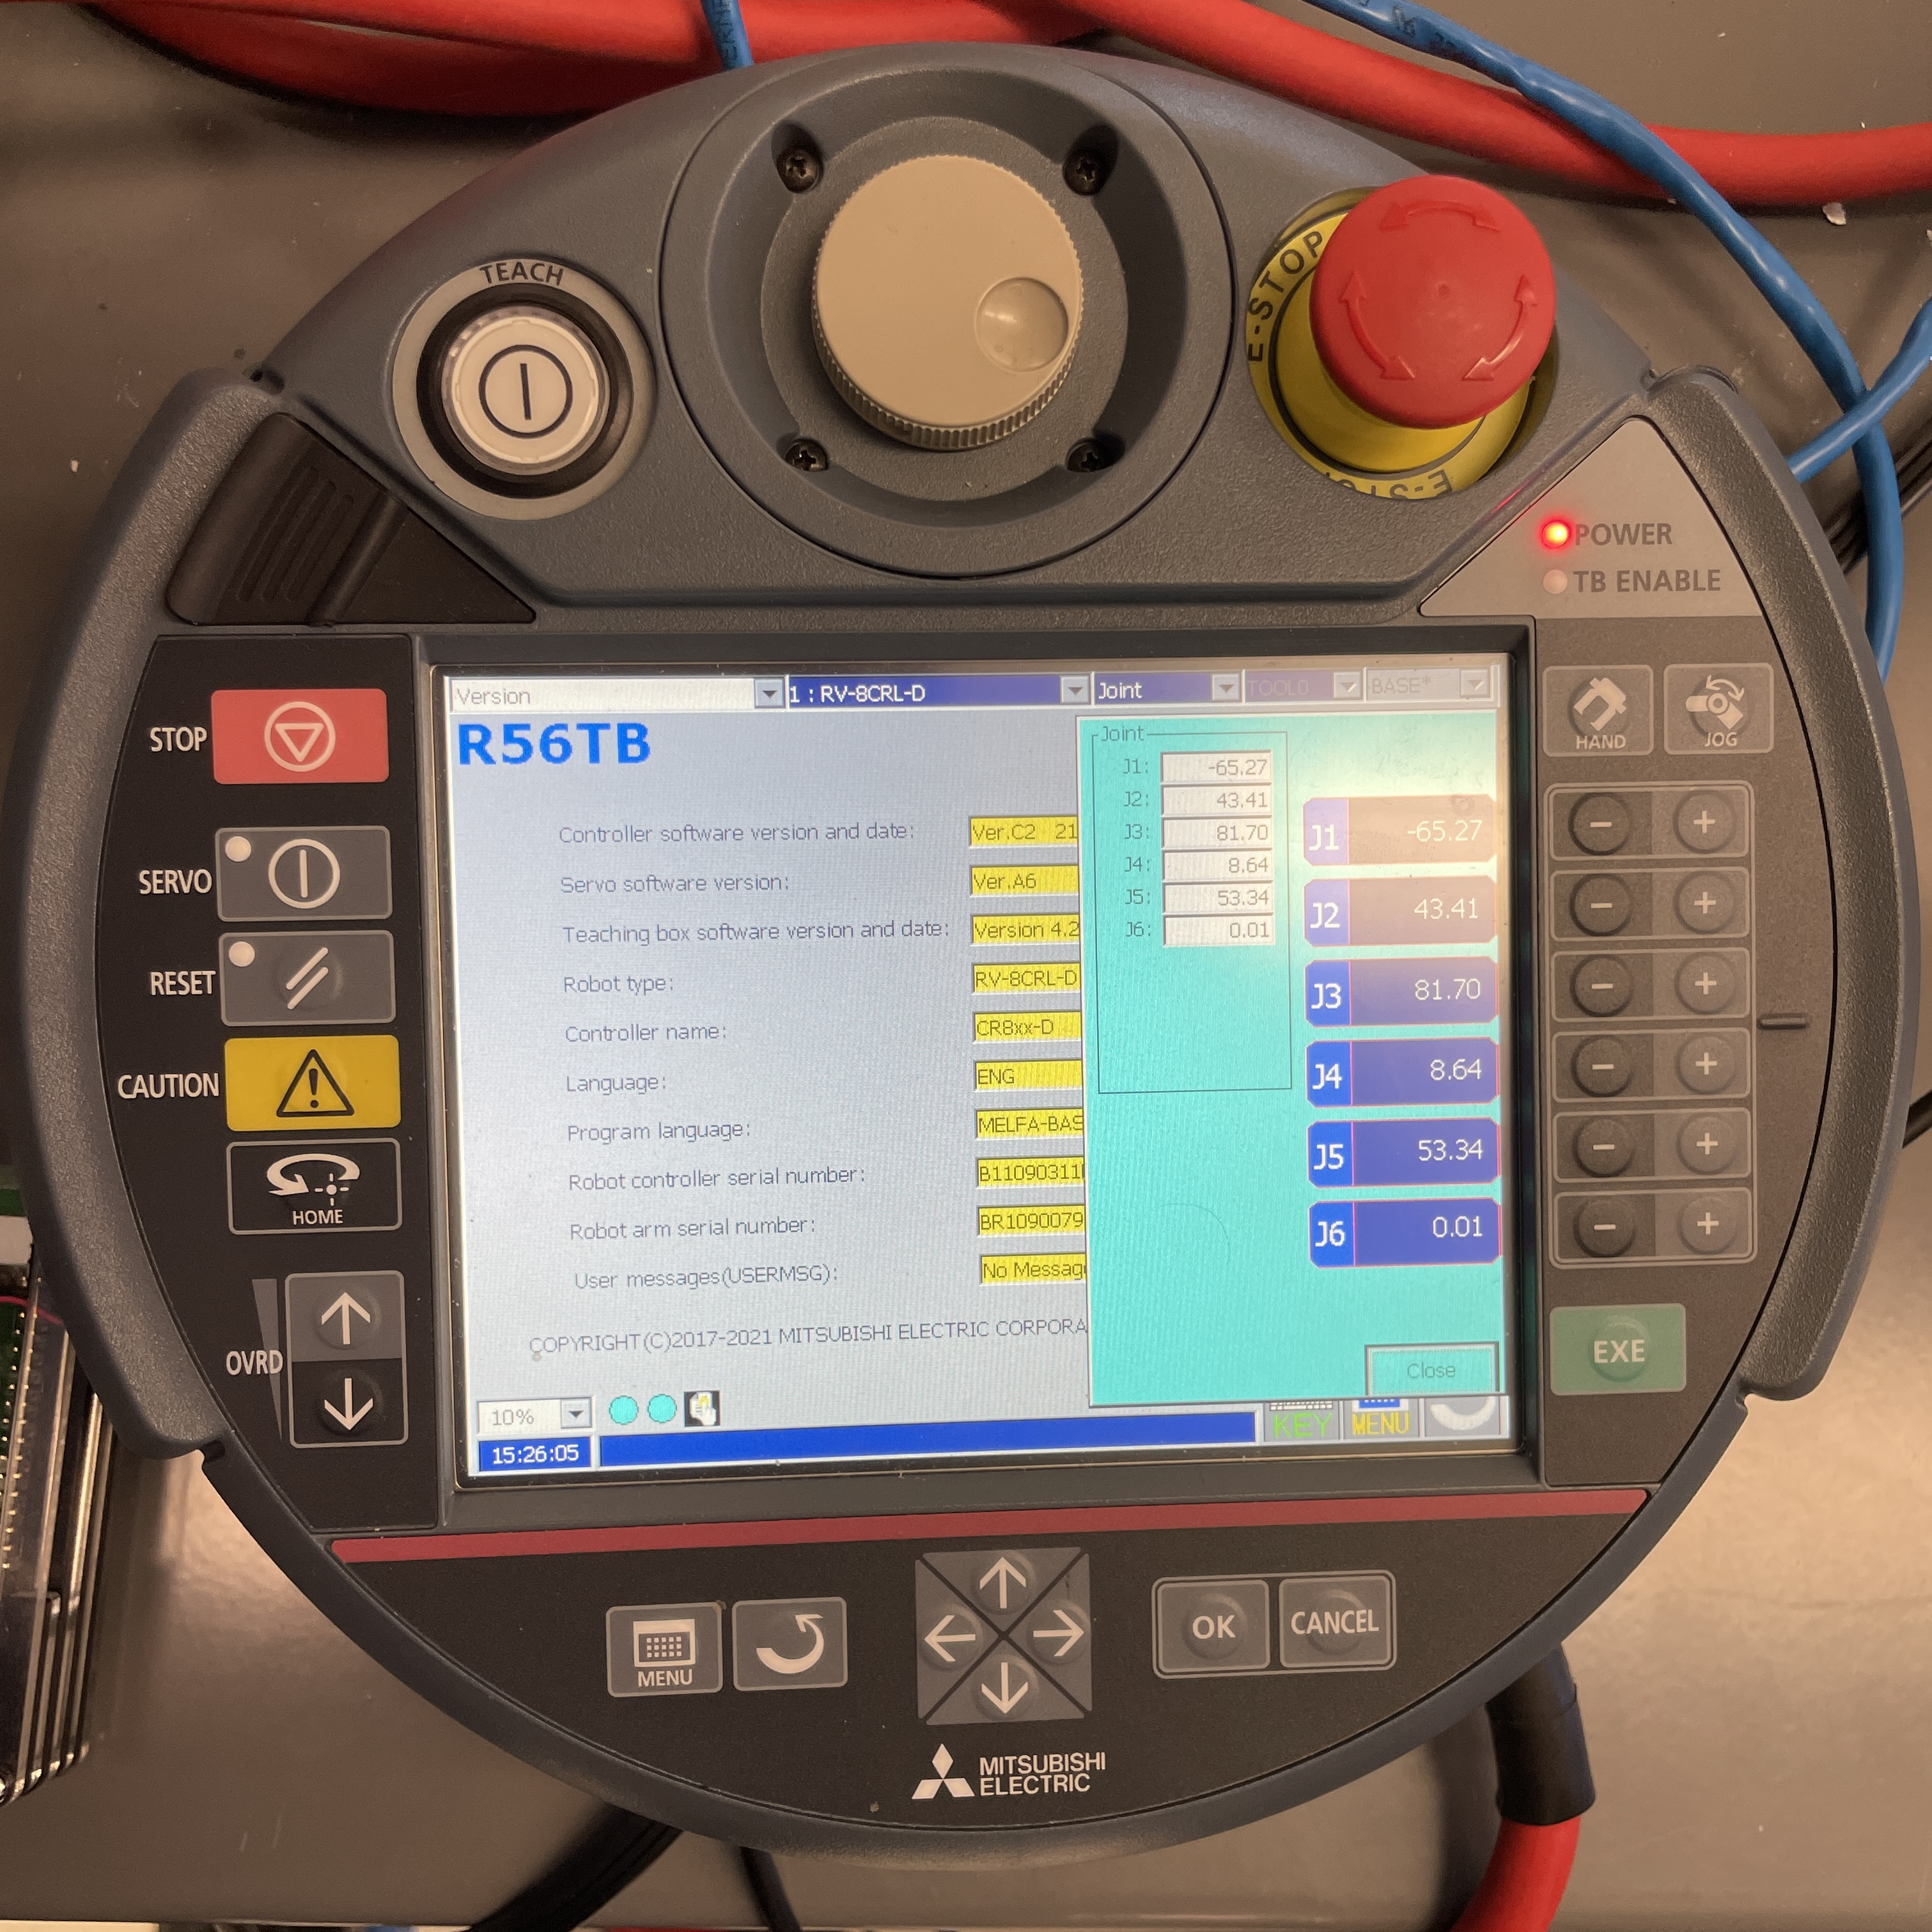
\includegraphics[width=0.40\textwidth]{images/CR800.jpg}
    \caption{CR800 controller}
\end{figure}



